\documentclass{article}

\usepackage{graphicx}
\usepackage{tikz}
\usepackage{tikzsymbols}
\usetikzlibrary{calc,patterns,shapes.geometric}
\pagestyle{empty}
\usepackage[margin=0pt]{geometry}
\geometry{papersize={14in,12in}}

\def\centerarc[#1](#2)(#3:#4:#5){\draw[#1] ($(#2)+({#5*cos(#3)},{#5*sin(#3)})$) arc (#3:#4:#5);}

\begin{document}
	\begin{figure}
		\centering
		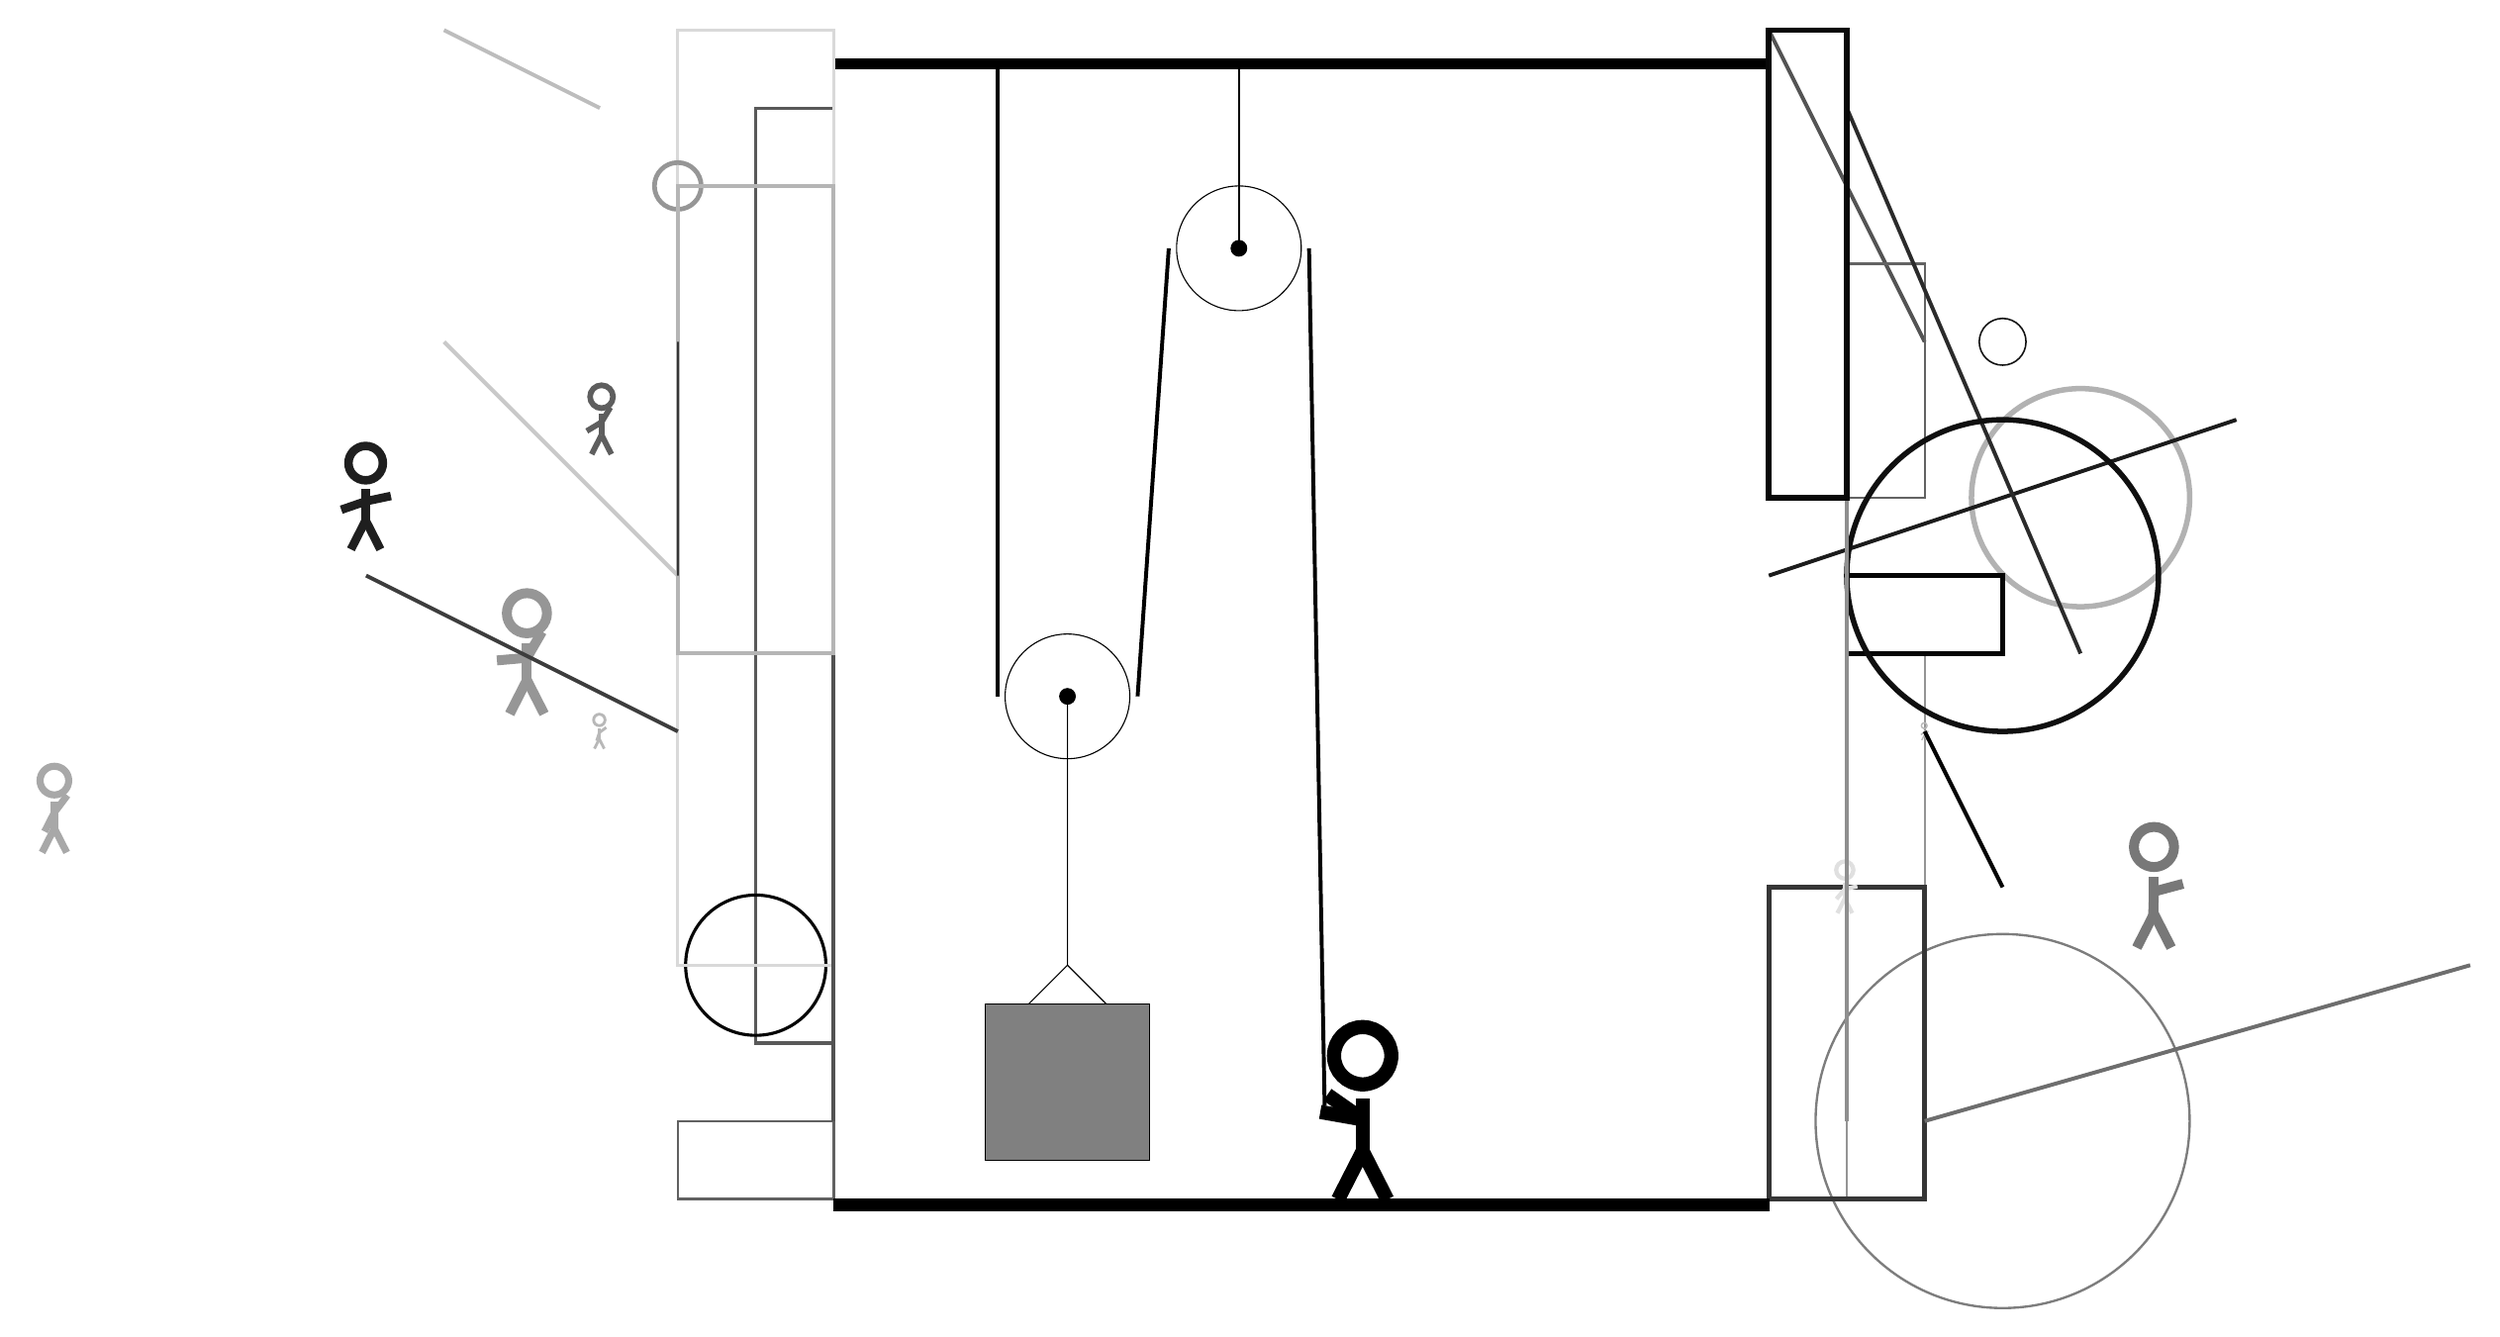
\begin{tikzpicture}
			%%%%% START %%%%%
			
			\draw[fill=black] (-2, 11.5) rectangle (10, 11.625);
			
			\draw (3.2, 9.2) circle (0.8);
			\draw[fill=black] (3.2, 9.2) circle (0.1);
			\draw[thick] (3.2, 9.2) -- (3.2, 11.5);
			
			\draw[line width=0.3mm, color=black!42] (12, -3) rectangle (11, 4);
			
			\draw [line width=0.7mm, color=black!30](14, 6) circle (1.4);
			\draw[line width=0.4mm, color=black!65] (-3, 11) rectangle (-2, -1);
			\draw[line width=0.5mm, color=black!67](10, 12) -- (12, 8);
			
			\draw[line width=0.3mm, color=black!62] (-2, -2) rectangle (-4, -3);
			
			\draw [line width=0.3mm, color=black!51](13, -2) circle (2.4);
			\draw [line width=0.4mm, color=black!98](-3, 0) circle (0.9);
			\draw[line width=0.6mm, color=black!79] (12, 1) rectangle (10, -3);
			\draw[line width=0.3mm, color=black!61] (11, 6) rectangle (12, 9);
			\node[line width=0.4mm, color=black!53] at (15, 1) {\Strichmaxerl[7][88][15]};
			
			\node[line width=0.6mm, color=black!28] at (-5, 3) {\Strichmaxerl[2][72][37]};
			
			\draw[line width=0.5mm, color=black!21](-7, 8) -- (-4, 5);
			\node[line width=0.4mm, color=black!63] at (-5, 7) {\Strichmaxerl[4][31][59]};
			
			\draw[line width=0.5mm, color=black!89](10, 5) -- (16, 7);
			\draw[line width=0.4mm, color=black!15] (-2, 12) rectangle (-4, 0);
			\draw[line width=0.5mm, color=black!57](12, -2) -- (19, 0);
			
			\node[line width=0.4mm, color=black!12] at (11, 1) {\Strichmaxerl[3][50][13]};
			\draw [line width=0.6mm, color=black!41](-4, 10) circle (0.3);
			\draw[line width=0.6mm, color=black!98] (11, 5) rectangle (13, 4);
			
			\node[line width=0.7mm, color=black!88] at (-8, 6) {\Strichmaxerl[6][19][12]};
			\draw[line width=0.5mm, color=black!83](14, 4) -- (11, 11);
			
			\draw [line width=0.7mm, color=black!94](13, 5) circle (2.0);
			\node[line width=0.6mm, color=black!28] at (12, 3) {\Strichmaxerl[1][39][9]};
			\draw[line width=0.5mm, color=black!68](-2, 8) -- (-2, -2);
			\draw[line width=0.5mm, color=black!44](11, 8) -- (11, -2);
			\node[line width=0.3mm, color=black!41] at (-6, 4) {\Strichmaxerl[7][5][60]};
			\draw[line width=0.5mm, color=black!29] (-2, 10) rectangle (-4, 4);
			\draw[line width=0.5mm, color=black!26](-7, 12) -- (-5, 11);
			\draw[line width=0.3mm, color=black!79] (-4, 8) rectangle (-4, 5);
			
			\node[line width=0.7mm, color=black!34] at (-12, 2) {\Strichmaxerl[5][63][53]};
			\draw[line width=0.5mm, color=black!99](12, 3) -- (13, 1);
			
			\draw[line width=0.5mm, color=black!76](-4, 3) -- (-8, 5);
			\draw [line width=0.2mm, color=black!93](13, 8) circle (0.3);
			\draw[line width=0.7mm, color=black!97] (11, 12) rectangle (10, 6);
			
			
			\draw (1, 3.45) circle (0.8);
			\draw[fill=black] (1, 3.45) circle (0.1);
			
			\draw (1, 3.45) -- (1, 0.0) -- (0.5, -0.5);
			\draw (1, 0.0) -- (1.5, -0.5);
			\draw[fill=black!50] (-0.05, -0.5) rectangle (2.05, -2.5);
			
			\draw[line width=0.5mm] (0.1, 11.5) -- (0.1, 3.45);
			\centerarc[line width=0.5mm](1, 3.45)(180:360:0.9);
			\draw[line width=0.5mm](1.9, 3.45) -- (2.3, 9.2);
			\centerarc[line width=0.5mm](3.2, 9.2)(0:180:0.9);
			\draw[line width=0.5mm](4.1, 9.2) -- (4.3, -1.8);
			
			\node at (4.7, -1.9) {\Strichmaxerl[10][-35][170]};
			
			\draw[fill=black] (-2, -3) rectangle (10, -3.15);
			
			%%%%% END %%%%%
		\end{tikzpicture}
	\end{figure}	
\end{document}